\subsection{Finite-budget local optimization at ten facets}
\label{subsec:black-box-datascience-finite-budget-optimization}

The random-table scan does not ask how far a local method can improve one
polytope.  We therefore compared seven iterative optimizers on \(64\)
previously unused random ten-facet starting points.  The starts were disjoint
from the development and tuning populations.  Every run received the same
\(1000\)\,ms measured serial-compute budget, including full evaluations of the
systolic ratio and the optimizer's own work, together with a cap of \(128\)
full evaluations.  The manifest fixed all methods and hyperparameters before
the held-out outcomes were computed.

The methods are standard gradient, derivative-free, and population ideas
\cite{NocedalWright2006}, adapted to the lower-envelope structure
\[
  \operatorname{sys}(a)=\min_\sigma s_\sigma(a).
\]
Here \(s_\sigma\) is a smooth KKT branch only on its branch domain, and the
minimizing word and admissible branch set can change with \(a\).  Thus the
gradient of one minimizing branch need not ascend the lower envelope.  The
model \(f(x,y)=y-|x|\) already shows the issue: at its ridge, either selected
branch gradient points away from the ridge, while balancing both branches
gives the ascending direction along it.

All local methods propose in the \(25\)-dimensional Euclidean slice transverse
to translations, common scaling, and the linear symplectic action.  Every
proposed outer step is then checked by a fresh geometry reconstruction and
global orbit-word search for \(\operatorname{sys}\).  Table
\ref{tab:black-box-datascience-f10-optimizer-steps} states the actual frozen
steps; it does not claim that the chosen parameters are optimal for their
algorithm families.

\begingroup
\small
\begin{longtable}{@{}p{0.24\linewidth}p{0.67\linewidth}@{}}
\caption{One outer iteration of each held-out optimizer.}
\label{tab:black-box-datascience-f10-optimizer-steps}\\
\toprule
method & implemented step\\
\midrule
\endfirsthead
\toprule
method & implemented step\\
\midrule
\endhead
literal and safeguarded
branch gradients
& Differentiate one currently minimizing branch.  The literal method takes
  the fixed update \(a^+=a+0.01D_as_\sigma(a)\) and continues even after a
  decrease.  The safeguarded method projects and normalizes this gradient,
  accepts only a fully evaluated improvement, and expands or halves its
  distance after acceptance or rejection.\\
finite-gap affine model
& Keep the current branch gaps in a \(10\%\) action window, linearize their
  values, and maximize the minimum affine value on a local ball.  Fully
  evaluate the proposal and use the same expand-or-halve distance rule.\\
four-anchor branch history
& Union candidate words from the four most recent full searches.  At a nearby
  point, re-solve the named KKT branches, retain the admissible ones, linearize
  their new values, and maximize their affine minimum.  Take at most two such
  internal moves before the next full evaluation.\\
history with transition prediction
& Use the preceding method, but for a normalized internal move of length at
  least \(0.08\), also predict newly feasible transitions in the move
  direction and evaluate the words thereby generated.\\
CMA-ES
& Fully evaluate a population of eight Gaussian perturbations, then update
  the mean, covariance, and normalized scale from their ranking.\\
coordinate direct search
& Poll both signs of the \(25\) transverse basis axes.  Move to the best
  improvement and double the radius, or halve the radius if no poll point
  improves.\\
\bottomrule
\end{longtable}
\endgroup

\begin{table}[htbp]
\centering
\scriptsize
\begin{tabular}{lrrr}
\toprule
method & median best \(\operatorname{sys}\) & 10--90\% across starts & maximum\\
\midrule
four-anchor branch history & \(0.9848\) & \(0.9570\)--\(0.9985\) & \(0.999826\)\\
history with transition prediction & \(0.9816\) & \(0.9559\)--\(0.9940\) & \(0.999711\)\\
finite-gap affine model & \(0.9772\) & \(0.9482\)--\(0.9946\) & \(0.997276\)\\
literal branch gradient & \(0.8813\) & \(0.7895\)--\(0.9239\) & \(0.948214\)\\
safeguarded branch gradient & \(0.8551\) & \(0.7804\)--\(0.9160\) & \(0.937475\)\\
CMA-ES & \(0.8183\) & \(0.7184\)--\(0.8692\) & \(0.932069\)\\
coordinate direct search & \(0.6010\) & \(0.3583\)--\(0.7866\) & \(0.842539\)\\
\bottomrule
\end{tabular}
\caption{Held-out outcomes on \(64\) matched random ten-facet starts at equal
measured serial compute.  The intervals describe variation across starting
points, not uncertainty about the median.}
\label{tab:black-box-datascience-f10-optimizer-comparison}
\end{table}

\begin{figure}[htbp]
\centering
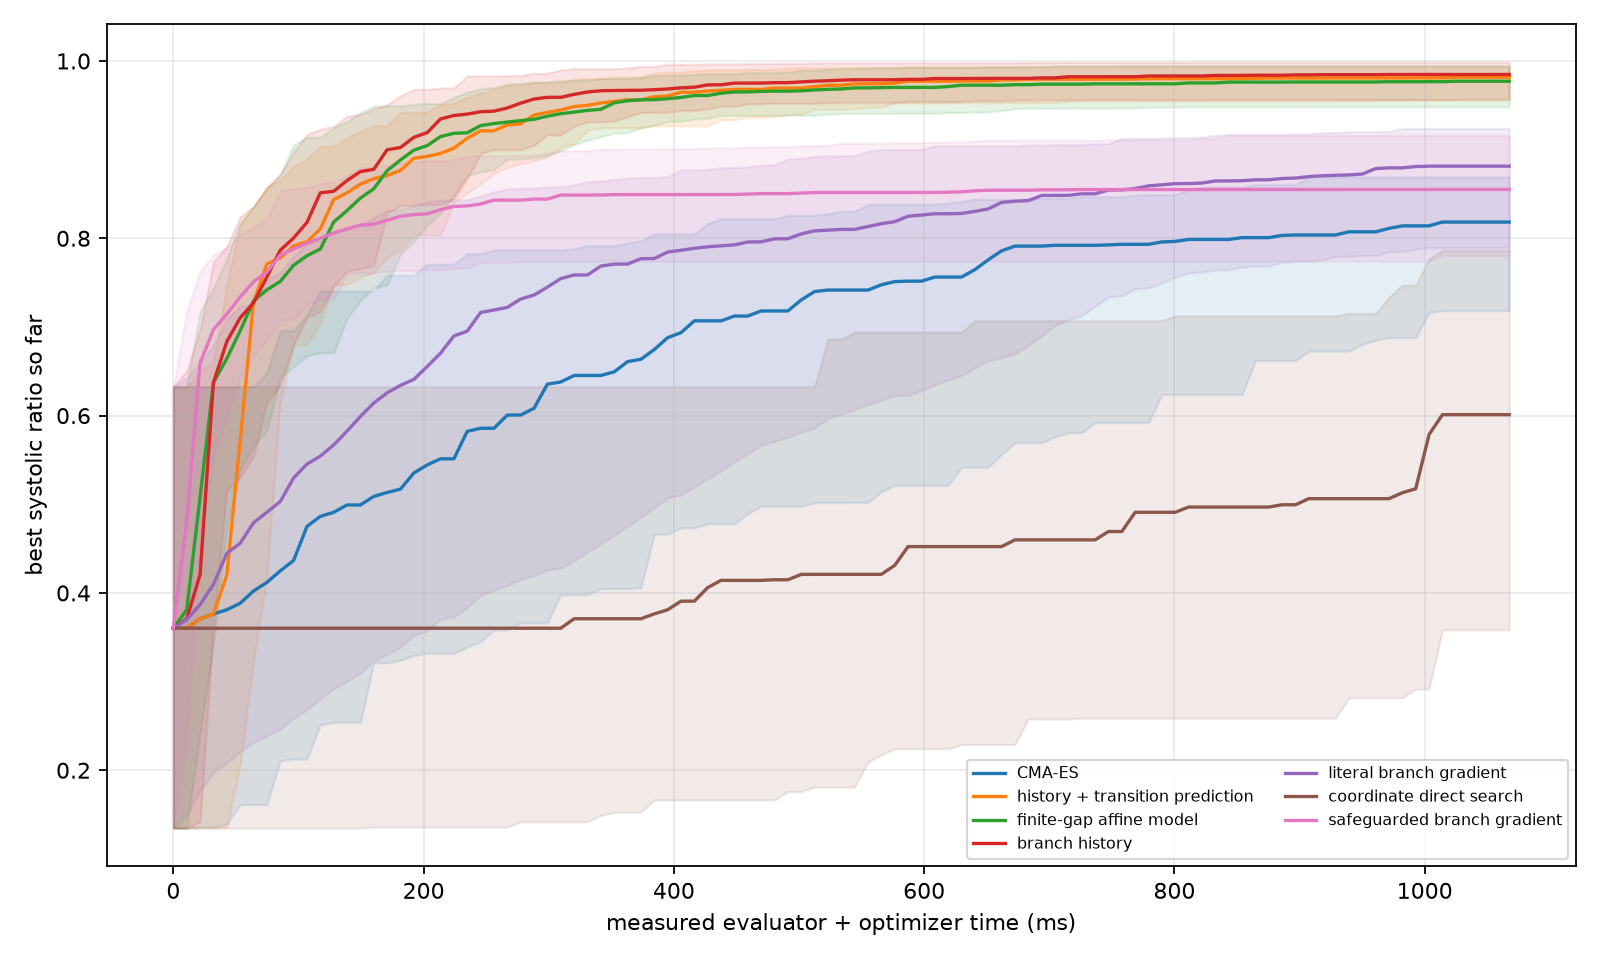
\includegraphics[width=0.96\linewidth]
  {../experiments/dev-gradient-ascent/optimizer-comparison/artifacts/heldout-f10-64-finalists-19a8b4dfd-analysis/figures/best-sys-by-measured-compute.png}
\caption{Median best systolic ratio against measured
evaluator-plus-optimizer time.  Shaded bands show the 10--90\% range across
the same \(64\) starts.}
\label{fig:black-box-datascience-f10-optimizer-compute}
\end{figure}

The branch-history method has the largest held-out median.  On matched starts,
its median advantage over transition prediction is \(0.00333\), with bootstrap
interval \(0.000073\)--\(0.00824\).  The more elaborate transition rule had
improved the development population, but did not generalize as an overall
replacement.  The finite-gap model remains a strong independent baseline.
Both single-branch gradients, CMA-ES, and coordinate search are substantially
weaker at this budget.  No held-out run reached
\(\operatorname{sys}\geq1\).

The objective curves alone do not establish convergence.  CMA-ES, literal
gradient, and coordinate search are still visibly improving at the budget
boundary, while a branch-aware method can stop because its local model returns
no proposal or its internal distance becomes too small.  We therefore tested
\(16\) population-stratified branch-history endpoints in both signs of all
\(25\) transverse basis axes, at relative radii \(10^{-3}\), \(10^{-4}\), and
\(10^{-5}\).  Seven one-second endpoints had an explicit fully recomputed
improving direction.  Repeating the same starts with a five-second ceiling
changed seven endpoint values and reduced the count to two, so five failures
were ordinary insufficient-depth failures.

Passing this finite basis poll is only a necessary-condition check: ascent may
lie between the basis axes.  Indeed, a separate diagnostic followed a
branch-informed improving path from each of three deliberately selected
endpoints for ten validated steps, stopping only at the imposed step cap.  One
of these endpoints had no improving basis-axis probe, yet gained \(0.00223\)
over normalized path length \(0.01\) and still had positive tested slope
\(0.0620\).  These paths are lower bounds on remaining improvement, not
estimates of an eventual maximum.

We therefore select four-anchor branch history only as the strongest tested
finite-budget method for this random \(F=10\) population and one-second
budget.  The experiment neither proves convergence to a local maximum nor
transfers the ranking to another facet count, starting distribution, or
budget.  It also leaves open whether any other fixed-\(F\) local maximum has
systolic ratio larger than \(1\).
